%----------------------------------------------------------------------------
\chapter{Case Study}\label{sect:case-study}
In this section I want to demonstrate the functionalities of Model-based test generation. For this i have created a garage gate system. First I describe the common functionality of the system, then I set-up the system requirements and finally I introduce the implementation and design decisions of the system.

\section{System introduction}
The system is a garage gate, which consists of two gates, a lamp, a control switch, a control logic and a movement sensor. With the control switch we can open or close the gate. When someone or something got into the gate, while it is closing, the gate stops. Consequently if the gate is free again (nobody has been detected by the movement sensor) it can continue the closing session after some seconds long lamp lighting warning.

\section{Requirements}
\textbf{Control flow}

[REQ-01-1] The control switch should have an open and close button.
[REQ-01-2] The signal from the control switch should be reachable up to 200m.
[REQ-01-3] Open/Close control action must have ended in Opened/Closed state of the gate.

\textbf{Lamp}

[REQ-02-1] While the lamp is lighting the gate should not move.
[REQ-02-2] 

\textbf{Movement Sensor}

[REQ-03-1] The sensor must detect if anything is between the two pillars of the gate.
[REQ-03-2] If the sensor detect blocking thing in the gate, a blocking signal must be sent immediately to the Gate Logic.
[REQ-03-3] If the sensor does not detect anything in the gate, it must wait for 5 seconds and then send a free signal to the Gate Logic.

\textbf{Control Logic}

[REQ-04-1] The opening and closing movement must be started with a signal from the control switch.

%TODO write design details
\section{System realization}
%specific UML diagrams, component diagram or component composition diagram (like SWSV::RIS description)

The system consists  4 elements, which are shown on the \figref{Garage Component} figure. The \textit{Gate} element stands for the physical representation of the Garage Gate itself, and can be in \textit{Opened} and \textit{Closed} states. We can open and close the \textit{Gate} with a \textit{Remote Controller}. If we start an action we can not pause or stop that. Nevertheless there is a \textit{Movement Sensor} on the two pillars of the \textit{Gate}, which stops the movement. When the \textit{Gate} is opening and the \textit{Movement Sensor} observes an object between the two pillars, it stops the movement (\textit{Opening Blocked}), until the object is not there any more. In the other case, when the \textit{Gate} is closing and the \textit{Movement Sensor} sign appears, it stops the movement again (\textit{Closing Blocked}). When the object is outside of the scope of the \textit{Movement Sensor} a \textit{Lamp}s on the pillars are \textit{Lighting} for some seconds then the \textit{Gate} is closing again.
So the \textit{Lighting} comes only in the closing interruption.

\begin{figure}[!ht]
	\centering
	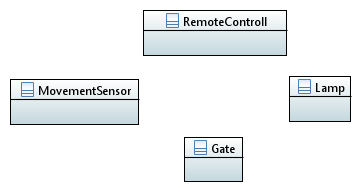
\includegraphics[width=100mm, keepaspectratio]{figures/component.png}
	\caption{Garage gate components}
	\label{fig:Garage Component}
\end{figure}

These components can communicate to each other directly. The possible communication messages is shown on the \figref{Garage communication}

\begin{figure}[!ht]
	\centering
	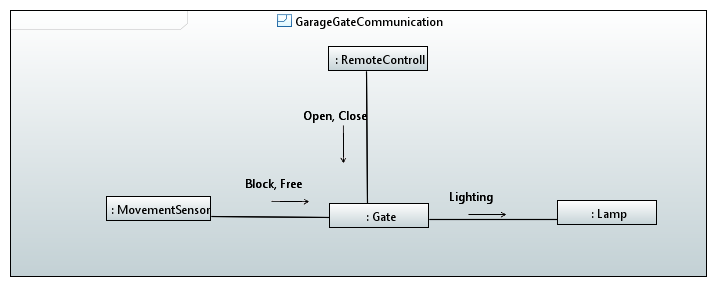
\includegraphics[width=150mm, keepaspectratio]{figures/communication.png}
	\caption{Garage gate communication diagram}
	\label{fig:Garage communication}
\end{figure}

A garage gate fundamentally have 2 main states, the \textit{Opened} and \textit{Closed} states, which is shown below on \figref{Garage Statemachine} figure, with orange colours.  First of all we can start from the \textit{Closed} state, where we can open the gate with an 'open' command. This command sets the state machine in an \textit{Opening} state. While opening the gate, somebody or something can move into the way, so this becomes \textit{Block Opening}. The gate is opening, if the blocking stops. After the \textit{Opening} phase succeeded the gate is \textit{Opened}. In this state we can 'close' the gate with a simple command, and the state machine goes to the \textit{Closing} state. There could be also a blocking action, which stops the closing movement. From this state the gate is starting the closing movement again after a few seconds \textit{Lighting}. When the closing action finished the gate is \textit{Closed}.



\begin{figure}[!ht]
\centering
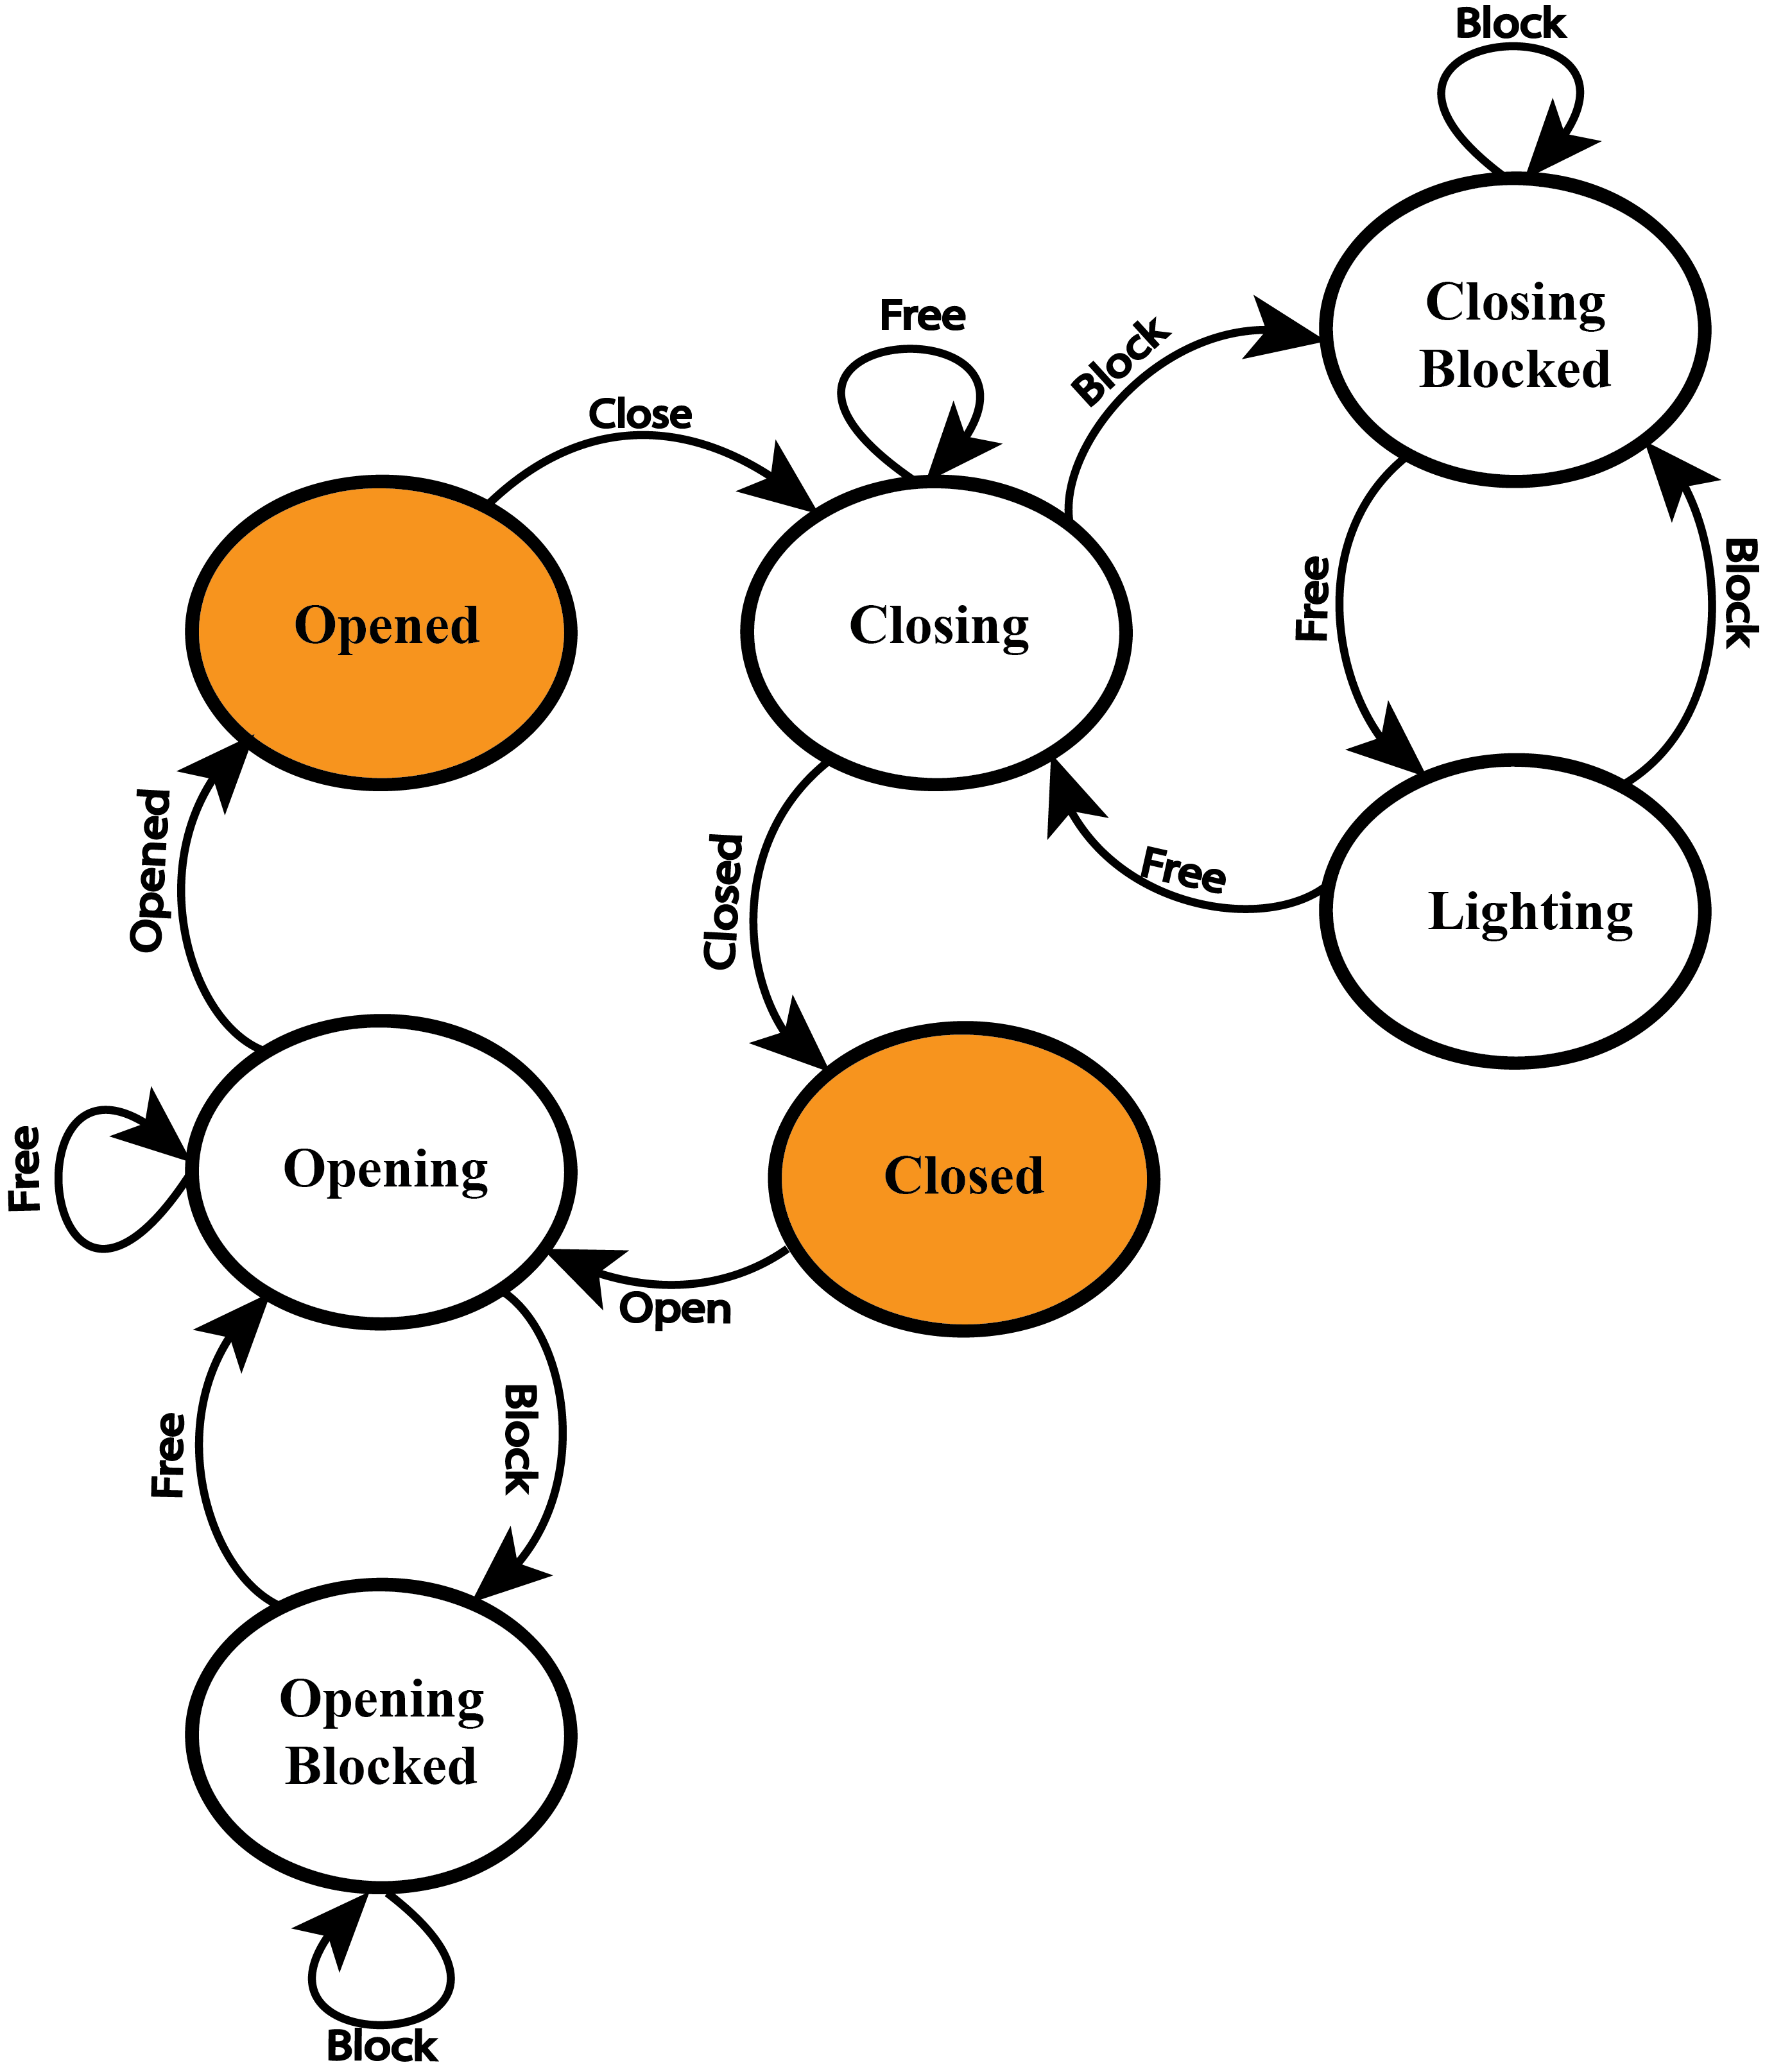
\includegraphics[width=150mm, keepaspectratio]{figures/garageState.png}
\caption{Garage gate state machine diagram}
\label{fig:Garage Statemachine}
\end{figure}

